%%%%%%%%%%%%%%%%%%%%%%%%%%%%%%%%%%%%%%%%%%%%%%%%%%%%%%%%%%%%%%%%%%%%%%%%%
% Antes de correr el código:
% 1. Ingresar al Menu
% 2. Cambiar la opción "Compiler" a XeLaTeX
% 3. Cambiar la opción "TeX live version" a 2020 (opacidad de la imagen)
%%%%%%%%%%%%%%%%%%%%%%%%%%%%%%%%%%%%%%%%%%%%%%%%%%%%%%%%%%%%%%%%%%%%%%%%%
\documentclass[10pt]{article}
\usepackage[T1]{fontenc}
\usepackage[utf8]{inputenc}
\usepackage[english]{babel}
\usepackage{listings}
\lstset{language=R}
\usepackage[a4paper]{geometry}
\usepackage[dvipsnames]{xcolor}
\usepackage[framemethod=TikZ]{mdframed}
\usepackage{graphicx,tikz}
\usepackage{array}
\usepackage{float}
\usepackage{tocloft}
\setlength{\cftsecnumwidth}{2em}

\geometry{top=2.54cm, bottom=2.54cm, left=2.54cm, right=2.54cm}

\usepackage{url}
\usepackage{lipsum} 
\usepackage{wrapfig}
\usepackage{subcaption}
\usepackage{multicol}

%==========================================
%======     FUENTE PARA CÓDIGOS      ======
%==========================================
\definecolor{codegreen}{rgb}{0,0.6,0}
\definecolor{codegray}{rgb}{0.1,0.1,0.1}
\definecolor{backcolour}{rgb}{0.98,0.98,0.98}

\lstdefinestyle{mystyle}{
  backgroundcolor=\color{backcolour},   
  commentstyle=\color{codegreen},
  keywordstyle=\color{blue},
  numberstyle=\tiny\color{codegray},
  stringstyle=\color{codegreen},
  basicstyle=\ttfamily\footnotesize,
  breakatwhitespace=false,         
  breaklines=true,                 
  captionpos=b,                    
  keepspaces=true,                 
  numbers=left,                    
  numbersep=5pt,                  
  showspaces=false,                
  showstringspaces=false,
  showtabs=false,                  
  tabsize=2
}

%==========================================
%==========     ESTILO TITLE     ==========
%==========================================
\newcommand{\City}[1]{\def\City{#1}}

\makeatletter         
\renewcommand\maketitle{
\begin{flushleft}
{\textcolor{black}{\huge \bfseries \@title }}\\[1ex]
\rule{\textwidth}{0.6pt}\\
\end{flushleft}
\vspace{-0.5cm}

\begin{flushleft}
\textcolor{black}{{\large  \@author} }\\[2ex]
\end{flushleft} } % Note the extra }
\makeatother

%==========================================
%==========    ESTILO CAPTION    ==========
%==========================================
\usepackage{caption}
\captionsetup[table]{name=Tabla ,textfont={it}, labelfont={bf},
                     justification=centering,
                     width =\dimexpr \textwidth-0.5cm\relax}
\captionsetup[figure]{textfont={it}, labelfont={bf},
                      justification=centering, skip=2pt,
                      belowskip=-5pt}
                      
%==========================================
%==========     ESTILO ITEM      ==========
%==========================================
\renewcommand{\labelitemi}{$\bullet$} 
\renewcommand{\labelitemii}{$\circ$} 
\renewcommand{\labelitemiii}{$\cdot$} 

%==========================================
%===    LINKS (Agregar Hyperlinks)     ====
%==========================================
\usepackage[style=apa,
            urldate=long]{biblatex} 
\addbibresource{Bib.bib}

\DeclareSourcemap{
  \maps[datatype=bibtex]{
    \map{
      \step[fieldsource=note, final]
      \step[fieldset=addendum, origfieldval, final]
      \step[fieldset=note, null]}
      }
}

\DefineBibliographyStrings{english}{urlseen = {Accessed }    
}

\usepackage[colorlinks=true,linkcolor=RoyalBlue,
            citecolor=RoyalBlue,urlcolor=RoyalBlue]{hyperref}

%==============================================================
%==============================================================
\title{ }

%%%%%%%%%%%%%%%%%%%%%%%%%%%%%%%%%%%%%%%%%%%%%%%%%%%%%%%%%%%%%%%
%%%%%%%%%%%%                 INICIO                %%%%%%%%%%%% 
%%%%%%%%%%%%%%%%%%%%%%%%%%%%%%%%%%%%%%%%%%%%%%%%%%%%%%%%%%%%%%%
\begin{document}

\begingroup
\let\clearpage\relax % prevent extra page breaks
\thispagestyle{empty}
\begin{center}
{\huge \bfseries Universidad de los Andes}

\vspace{25pt}
{\LARGE \bfseries Departamento de Ingeniería de Sistemas}

\vspace{15pt}

\includegraphics[width=100pt]{images/logo.png} 

\vspace{35pt}
{\LARGE \bfseries Laboratorio \#2: Análisis De Protocolos De La Capa De Aplicación}
\vspace{55pt}

{\Large \bfseries ISIS3204 - Infraestructura de Comunicaciones}


\vspace{100pt}
{\Large \bfseries Grupo 3: }

\end{center}

\begin{flushleft}
  \setlength{\parskip}{0pt}
  \setlength{\itemsep}{0pt}
  \hspace*{4cm}\large\bfseries Juan Esteban Quiroga - 202013216

  \hspace*{4cm}\large\bfseries Juan Manuel Rodriguez - 202013372

  \hspace*{4cm}\large\bfseries Andres Felipe Ortiz - 201727662
\end{flushleft}

\begin{center}
\vspace{60pt}

\Large\bfseries 2025-10
\end{center}

\mbox{}
\endgroup

\clearpage

\tableofcontents
\clearpage


\renewcommand{\thesection}{\arabic{section}}
\section*{Introducción}
\addcontentsline{toc}{section}{Introducción}
Lorem ipsum dolor sit amet, consectetur adipiscing elit. Sed nec tristique eros. Vestibulum ante ipsum primis in faucibus orci luctus et ultrices posuere cubilia curae; Pellentesque sit amet purus a sapien porta viverra. Cras in feugiat nisl. Mauris volutpat lorem in ligula dapibus, non aliquam eros tristique. Suspendisse potenti. Nunc laoreet augue ac viverra dictum. Integer mattis magna in nisi consequat, nec vehicula nulla dignissim. Ut nec aliquam libero. Sed eu nisl vitae mauris congue eleifend at nec urna.

%==============================================================
%=====================   8.1   ================================
%==============================================================
\renewcommand{\thesection}{8.\arabic{section}}
\setcounter{section}{0}
\section{Prueba ping}

Lorem ipsum dolor sit amet, consectetur adipiscing elit. Sed nec tristique eros. Vestibulum ante ipsum primis in faucibus orci luctus et ultrices posuere cubilia curae; Pellentesque sit amet purus a sapien porta viverra.


\begin{figure}[H]
    \centering
    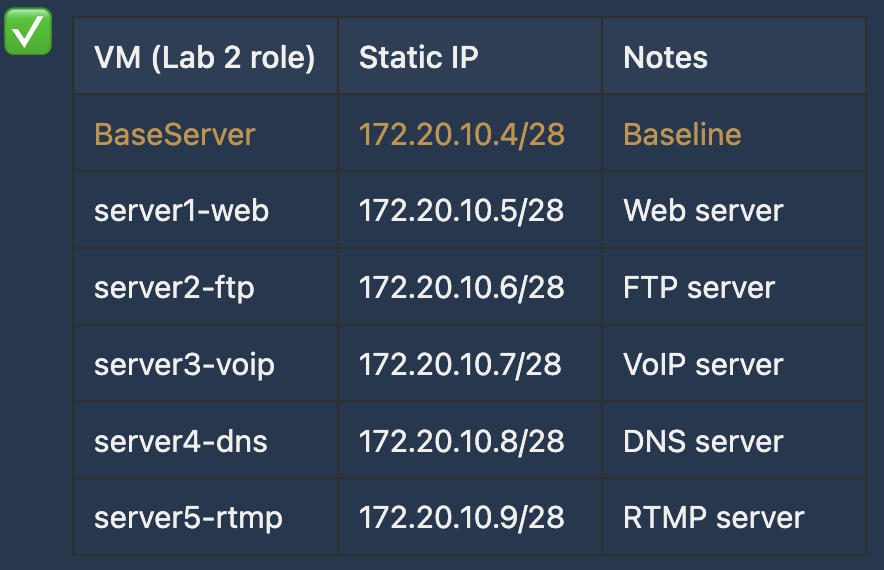
\includegraphics[width=0.65\textwidth]{lab-02-screenshots/server-ips.png}
    \caption{Configuración de IPs estáticas}
\end{figure}


\subsection{Prueba de conectividad al servidor DNS}
\subsection{Prueba de conectividad al servidor FTP}


%==============================================================
%=====================   8.2   ================================
%==============================================================
\renewcommand{\thesection}{8.\arabic{section}}
\section{Análisis de tráfico del Servicio DNS}
\subsection{Prueba de conectividad al Servidor Web (IP)}
\subsection{Prueba de conectividad al Servidor Web (URL)}


%==============================================================
%=====================   8.3   ================================
%==============================================================
\renewcommand{\thesection}{8.\arabic{section}}
\section{Análisis de tráfico del Servicio FTP}
\subsection{Conexión al servidor FTP}
\subsection{Descarga de archivo (Download)}
\subsection{Carga de archivo (Upload)}

%==============================================================
%=====================   8.4   ================================
%==============================================================
\renewcommand{\thesection}{8.\arabic{section}}
\section{Análisis de tráfico del Servicio Web}
\subsection{Acceso al servidor web mediante HTTP}

%==============================================================
%=====================   8.5   ================================
%==============================================================
\renewcommand{\thesection}{8.\arabic{section}}
\section{Análisis del protocolo HTTPS realizando navegación en el sitio de YouTube}
\subsection{Navegación en YouTube}
\subsection{Navegación en otros sitios HTTPS}
\subsubsection{https://www.elespectador.com}
\subsubsection{https://www.eltiempo.com}
\subsubsection{https://www.uniandes.edu.co}
\subsubsection{https://www.bancolombia.com}


%==============================================================
%=====================   8.6  ================================
%==============================================================
\renewcommand{\thesection}{8.\arabic{section}}
\section{Análisis del protocolo VoIP}
\subsection{Establecimiento de la llamada}


%==============================================================
%=====================   8.7   ================================
%==============================================================
\renewcommand{\thesection}{8.\arabic{section}}
\section{Análisis del protocolo RTMP}
\subsection{Inicio de la transmisión}


%==============================================================
%=====================   8.7   ================================
%==============================================================
\renewcommand{\thesection}{9.\arabic{section}}
\setcounter{section}{0}
\section{Topología}












\begin{thebibliography}{9}


  \bibitem{kurose_ross}
  Computer Networking, a top-down approach. James Kurose, Keith Ross. Addison-Wesley, 6th ed.

  \end{thebibliography}


\end{document}